\documentclass[crop,tikz]{standalone}
\usepackage{tikz,pgfplots}
\usetikzlibrary{calc,shapes}


\definecolor{coral}{RGB}{255,87,40}
\definecolor{cblue}{RGB}{31, 117, 254}
\definecolor{mantis}{RGB}{116, 195, 101}
\definecolor{shamrock}{RGB}{0, 158, 96}
\definecolor{emerald}{RGB}{80, 200, 120}
\definecolor{france}{RGB}{49, 140, 231}
\definecolor{gold}{RGB}{249,196,95}
\definecolor{klein}{RGB}{0,46,167}
\definecolor{ultramarine}{RGB}{63,0,255}
\definecolor{navy}{RGB}{0,0,128}
\definecolor{midnight}{RGB}{25,25,112}
\definecolor{burgundy}{RGB}{144, 0, 32}

%%%%%%%%%%%%%%%%%%%%%%%%%%%%%%%%%%%%%%%%%%%%%%%%%%%%%%%%%%%%
\colorlet{one}{gold}
\colorlet{two}{black!60!cblue}
% \colorlet{two}{midnight}
\colorlet{three}{gold!20}
\colorlet{four}{black!20!cblue!20}
\colorlet{five}{shamrock}


\colorlet{color_cite}{burgundy}
\colorlet{color_url}{navy}
\colorlet{color_link}{navy}


\tikzstyle{point}=[circle,scale=0.3,fill=black] 
\tikzstyle{cpoint}=[circle,scale=0.3,fill=red,draw=black] 

\begin{document}

  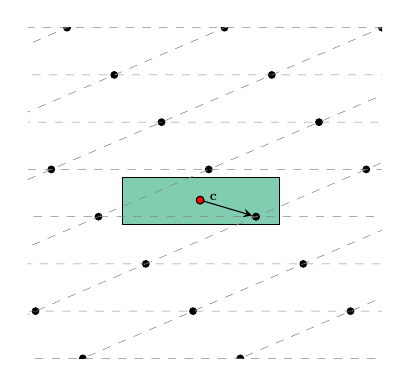
\begin{tikzpicture}[>=stealth]

        \clip (2.5,-1.2) rectangle (7cm,3cm);

      \node (c) at (4.7,.8) {};
      
       \fill[draw=black,fill=shamrock!50] ($(c)+(-1,-.3)$) rectangle ($(c)+(1,.3)$);
       \pgftransformcm{1}{0}{0.7}{0.3}{\pgfpoint{0cm}{0cm}};

      \node (c) at (2.8,2.7) {};
      \node (c) at (c) [cpoint] {};

      \node[color=black] at ($(c)+(.1,.1)$) [scale=0.5] {\textbf{c}};
      
        \foreach \x in {-4,-2,0,2,4,6,8,10} {
            \foreach \y in {-4,-2,0,2,4,6,8,10} {
                \node at (\x,\y) [point] {};
            }
        }

      
      \node (v) at (4,2) [point] {};
      \draw[->,black] (c) to (v);

        
      \draw[style=help lines,dashed] (-10,-10) grid[step=2cm] (14,14);


  \end{tikzpicture}

\end{document}

